%!TEX root = ../summaries.tex

\chapter{Learning from humans}

\section{Imitation Learning, Part 1}

\begin{itemize}
    \item Differences when moving from prediction to control for AI systems
    \begin{itemize}
        \item No longer i.i.d.
        \item From ground truth supervision to high-level, abstract goal.
        \item Objective: from predict label to accomplish task.
        \item In real world, some prediction systems also have feedback issues: e.g.\@ traffic prediction system used and affects traffic.
    \end{itemize}
    \item Terminology.
    \begin{itemize}
        \item $\bf o_t$: observation.
        \item $\bf a_t$: action.
        \item $\bf s_t$: state (underlying variables in model).
        \item $\pi_\theta(\bf a_t \mid \bf o_t)$ or $\pi_\theta(\bf a_t \mid \bf s_t)$: policy.
        \item When policy depends on state, it is \emph{fully observed}.
        \begin{figure}[h!]
            \centering
            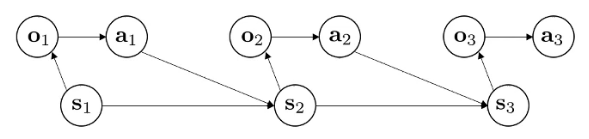
\includegraphics[width=.95\linewidth]{images/state-bayes-net.png}
            \caption{Bayes' net for the states, observations and actions}
            \label{fig:bayes net states}
        \end{figure}
    \end{itemize}
    \item Initiation learning: supervised learning.
    \begin{itemize}
        \item \emph{Behaviour cloning}.
        \item Doesn't work in theory: small mistakes compound, and we quickly diverge from training distribution.
        \item Works reasonably well in practice, given enough training data.
    \end{itemize}
\end{itemize}